\graphicspath{{./chapitres/chapitre3/figures/}}
\setcounter{mtc}{3}
\chapter{Sprint Un:  mise en place du protocole de communication avec le moteur graphique }
\fancyhead[R]{\ungaramond\small\textbf{Chapitre 3: mise en place du protocole de communication avec le moteur graphique }}
\minitoc
\newpage
\section*{Introduction}
Nous entamons le premier sprint de ce projet, nous allons mettre en relief les concepts clés tels que le but de ce sprint, son backlog et les étapes afin d’aboutir aux objectifs.


\section{Sprint\textcolor{white}{J}Backlog}
\subsection{Histoires\textcolor{white}{J}à\textcolor{white}{J} réaliser\textcolor{white}{J}pour\textcolor{white}{J}le\textcolor{white}{J}premier\textcolor{white}{J}Sprint}
Le\textcolor{white}{J}tableau\textcolor{white}{J} \ref{tab:tab-s1} \textcolor{white}{J} décrit\textcolor{white}{J} les\textcolor{white}{J} histoires\textcolor{white}{J} de\textcolor{white}{J} notre\textcolor{white}{J} backlog\textcolor{white}{J} du\textcolor{white}{J} premier\textcolor{white}{J} sprint.
\begin{longtable}[!ht]{|m{1cm}|m{3cm}|m{1cm}|m{7cm}|m{1.3cm}|}
\hline
{\textbf{Id story}} & {\textbf{User story}} & {\textbf{id tâche}} & {\textbf{tâche}} & {\textbf{estima-tion(H)}}\\
\hline
1.1 & En tant qu’utilisateur je souhaite recevoir les images synthétisées en temps  réel & 1.1.1 & Mettre en place le protocole de communication  & 6\\
\cline{3-5}
&   & 1.1.2 & Récupérer les images du moteur graphique en base64 & 6\\
\cline{3-5}
&   & 1.1.3 & Recevoir une qualité améliorée des images synthétisées & 4\\
\cline{3-5}
&	& 1.1.4 & Améliorer la fiabilité du flux & 4\\
\hline
\caption{Liste\textcolor{white}{J}des\textcolor{white}{J}tâches\textcolor{white}{J}du\textcolor{white}{J}premier\textcolor{white}{J}Sprint}
\label{tab:tab-s1}
\end{longtable}

\newpage
\section{Conception}
\subsection{Diagramme\textcolor{white}{J}d’activité\textcolor{white}{J}de\textcolor{white}{J}la\textcolor{white}{J}communication avec le moteur\textcolor{white}{J}graphique }

Le\textcolor{white}{J}diagramme\textcolor{white}{J}d’activité\textcolor{white}{J}dans\textcolor{white}{J}la figure \ref{fig:actEspClient}\textcolor{white}{J}représente\textcolor{white}{J}les\textcolor{white}{J}activités\textcolor{white}{J}possibles lors de la communication\textcolor{white}{J}avec\textcolor{white}{J}le\textcolor{white}{J}moteur\textcolor{white}{J}graphique.

\begin{figure}[!ht]\centering
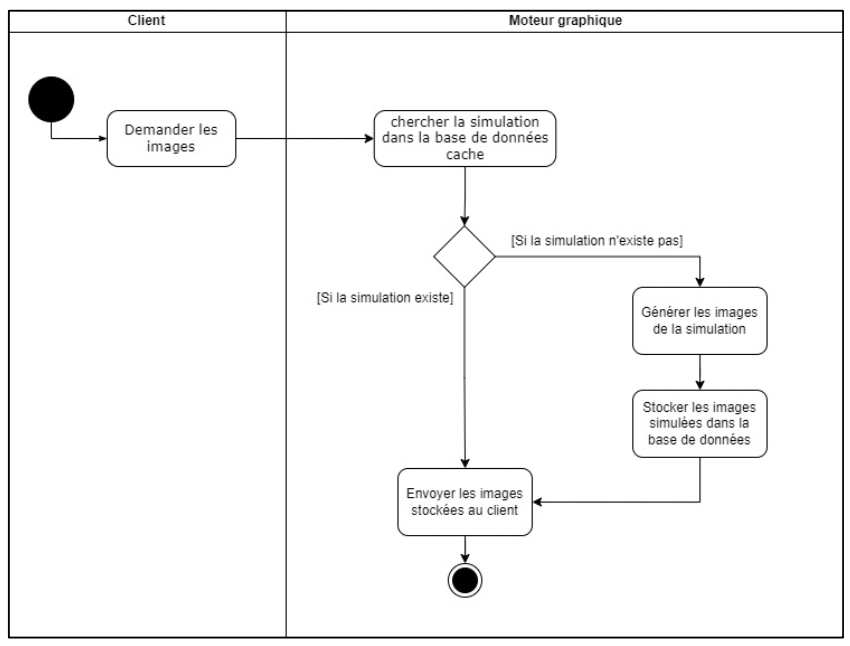
\includegraphics[width=1\textwidth,angle=00]{chapitres/chapitre3/figures/DiagAct-Moteur.png}
\caption{Diagramme\textcolor{white}{J}d'activité}
\label{fig:actEspClient}
\end{figure}

Lorsque le client demande les images synthetisées,le moteur graphique recherche la couleur demandée dans la base de données cache.Si la couleur existe,le moteur graphique va retourner les images récupérées au client.Sinon,il va procéder la la generation des images puis les stocker dans la base de donées cache et ensuite les retourner au client.

\newpage
\subsection{Diagramme\textcolor{white}{J}de\textcolor{white}{J}séquence\textcolor{white}{J}objet}
Le diagramme\textcolor{white}{J}de\textcolor{white}{J}séquence\textcolor{white}{J}objet\textcolor{white}{J}dans la figure \ref{fig:seqobj} représente les scénarios possibles et le comportement des objets\textcolor{white}{J}lors du la\textcolor{white}{J}communication\textcolor{white}{J}avec le moteur graphique.
\begin{figure}[!ht]
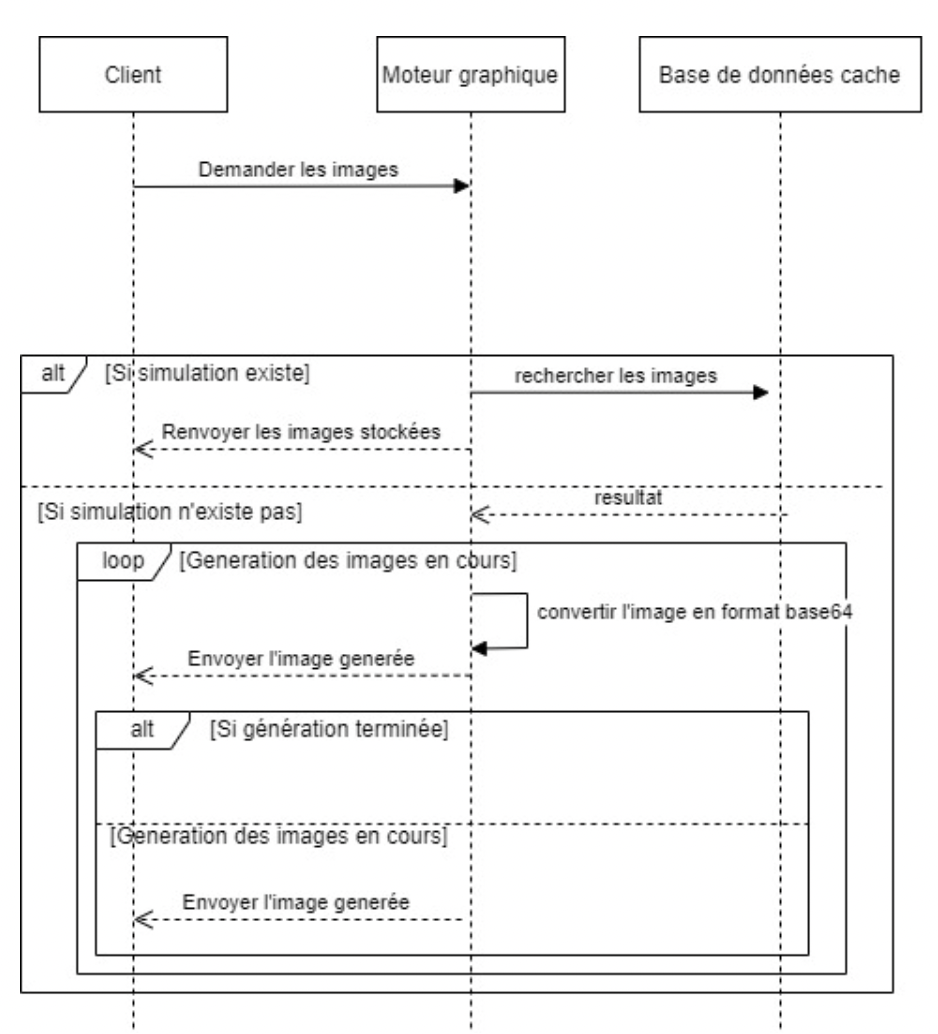
\includegraphics[width=0.8\textwidth,angle=00]{chapitres/chapitre3/figures/DiagSeqObj.png}
\caption{Diagramme\textcolor{white}{J}de\textcolor{white}{J}séquence\textcolor{white}{J}objet}
\label{fig:seqobj}
\end{figure}

Lorsque le client demande les images synthetisées,le moteur graphique recherche la couleur demandée dans la base de données cache.Si la couleur existe,le moteur graphique va retourner les images récupérées au client.Sinon,il va procéder la la generation des images puis les stocker dans la base de donées cache et ensuite les retourner au client.

\newpage
\subsection{Le format du protocole de communication}
On a mis en place un protocole de communication entre le moteur graphique et la partie backend.Le client doit demander les images de teinte en envoyant un format spécifique au moteur graphique ou on doit spécifier le type des cheveux, la couleur de base ainsi que la couleur de teinte et enfin les paramètres des caméras qui caractérise les quatre vues : vue de face, vue d’arrière, vue de dessus, vue de droite. 
La figure \ref{fig:figJSON} représente le protocole en format JSON.

\begin{figure}[!ht]
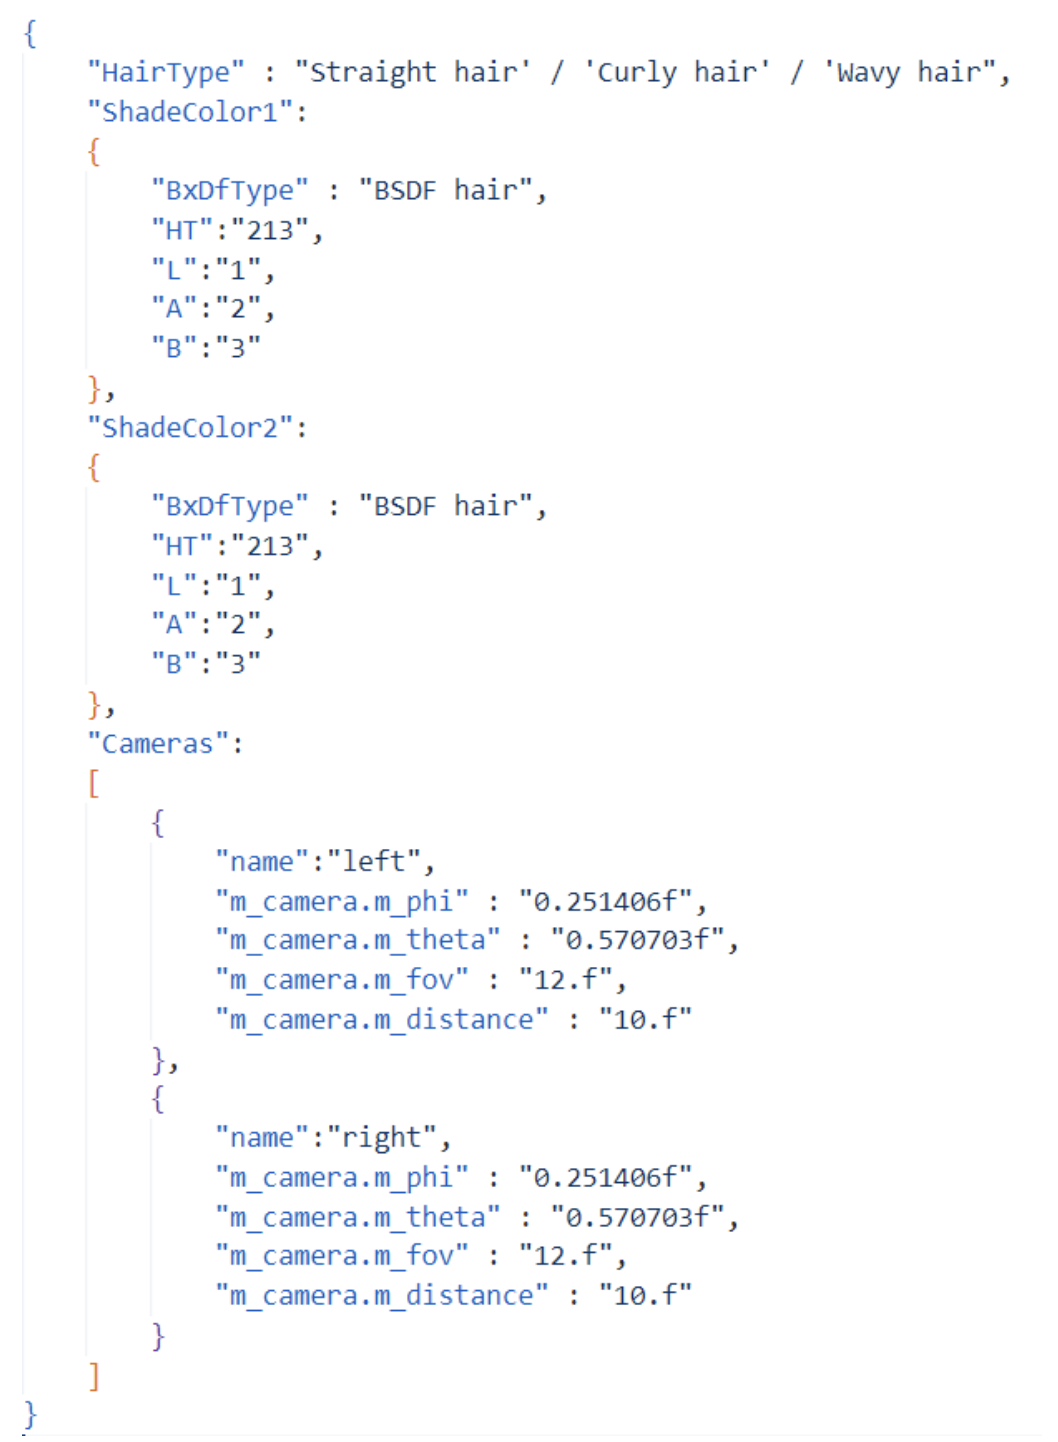
\includegraphics[width=0.8\textwidth,angle=00]{chapitres/chapitre3/figures/JSON.png}
\caption{Le protocole en format JSON}
\label{fig:figJSON}
\end{figure}

\newpage
Pour avoir les images synthétisées, le moteur graphique va extraire les images du modèle 3D puis les encoder avec l’encodage base64.Ces derniers vont être renvoyés au client avec une fréquence d’une image chaque deux secondes.

Le moteur graphique va ensuite améliorer progressivement la qualité des images et les envoyer au client.
La figure \ref{fig:figImage} représente le format de retour des images. 

\begin{figure}[!ht]
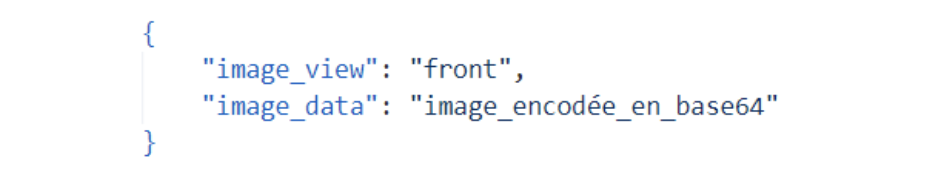
\includegraphics[width=0.8\textwidth,angle=00]{chapitres/chapitre3/figures/JSON-2.png}
\caption{Le format de retour des images}
\label{fig:figImage}
\end{figure}


\section{Réalisation}
\subsection{Technologies}
\subsubsection*{NVIDIA OptiX Ray-tracing Sdk[8]}
NVIDIA OptiX est un cadre d'application pour des performances optimales de traçage de rayons sur le GPU qui est utilisé pour la production de films et de vidéos ainsi que de nombreuses autres applications graphiques professionnelles. OptiX SDK 7.1 est la dernière mise à jour de la nouvelle API OptiX 7. La version 7.1 introduit une nouvelle primitive de courbe pour les cheveux et la fourrure et un débogage et un profilage améliorés.

\subsubsection*{WebSockets [9]}
WebSocket est un standard du Web désignant un protocole réseau de la couche application et une interface de programmation du World Wide Web visant à créer des canaux de communication full-duplex par-dessus une connexion TCP pour les navigateurs web. Avec cette technologie nous pouvons envoyer des messages à un serveur et recevoir ses réponses de manière événementielle sans avoir à aller consulter le serveur pour obtenir une réponse.

\subsubsection*{WebSocket++ (Zaphoyd/websocketpp) [10]}
WebSocket++ est une bibliothèque C++ qui implémente RFC6455 le protocole webSocket. Il permet d'intégrer les fonctionnalités client et serveur WebSocket dans les programmes C++.dans notre contexte on a implémenter la fonctionnalité serveur WebSocket. 

\subsection{Implémentation}
\subsubsection{l’Etat actuel de l’application}
Pour obtenir les images synthétisées des teintes, l’équipe digitale a développé une application de rendu graphique qui permet de simuler différentes nuances sur les cheveux en temps réel grâce a des algorithmes de Ray Tracing. La solution, intitulé OptixHair, a été basé sur l'API NVIDIA OptiX 7.5 qui est un cadre d'application permettant d'obtenir des performances optimales de traçage de rayons sur le GPU (Ray Tracing). Il s'agit d'une API de traçage de rayons. Les calculs sont déchargés sur les GPU via l'API de bas niveau ou de haut niveau introduite avec CUDA.
Cette solution est développée avec le langage de programmation C++. Elle est considérée comme solution client lourd (un logiciel installé sur un ordinateur) et nécessite une machine avec des spécifications particulières.

\begin{figure}[!ht]\centering
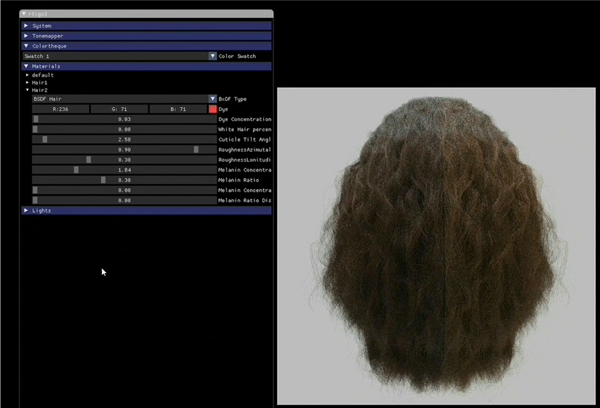
\includegraphics[width=0.6\textwidth]{chapitres/chapitre3/figures/old.png}
\caption{Client lourd} 
\label{fig:ec1}
\end{figure}

\newpage
\subsubsection{Evolution de l’application }
Pour mieux exploiter l’application OptixHair et permettre une large utilisation la solution envisagée consiste à transformer l’application en un moteur graphique qui reçoit des paramètres via un bus de communication instantanée précisant les caractéristiques de la teinte en vue de produire et envoyer des images synthétisées avec des améliorations continues toutes les deux secondes
La figure \ref{fig:mgraphique} ci-dessous représente le moteur graphique 

\begin{figure}[!ht]\centering
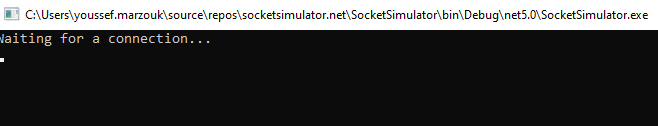
\includegraphics[width=0.6\textwidth]{chapitres/chapitre3/figures/console.png}
\caption{moteur graphique} 
\label{fig:mgraphique}
\end{figure}

\subsubsection{L’amélioration de la fiabilité et la rapidité du flux des images }
La rapidité de production des images par le moteur graphique peut engendrer des anomalies, voir même des images non accomplies. Pour cela, il a été convenu de repérer les deux bouts de l’images en ajoutant un caractère spécial dans chaque extrémité.
Chaque simulation produite par le moteur graphique est stockée dans une base de données qui peut être consultée par le moteur graphique en cas de besoin, et ce pour gagner du temps et augmenter la performance du moteur graphique.


\section*{Conclusion}
Ce sprint a abouti à la mise en place du protocole de communication et compréhension de l’objectif final du projet. Ce résultat est fondamental pour réaliser les autres sprints.


